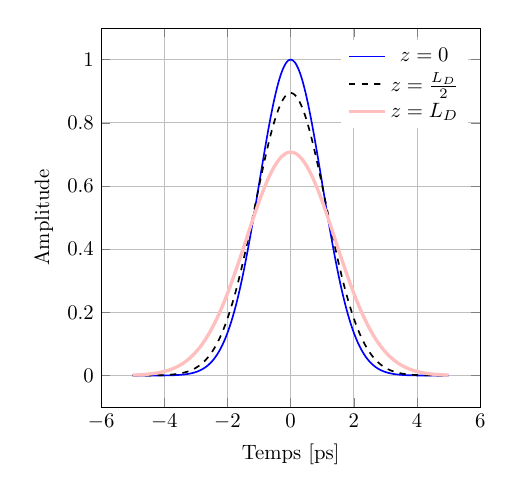
\begin{tikzpicture}[scale = 0.75]
	\begin{axis}[
		width       = 8cm,
		height      = 8cm,
		xlabel      = {Temps [ps]},
		ylabel      = {Amplitude},
		legend pos  = north east,
		legend style= {draw=none},
		grid        = major
	]

        % z = 0
        \addplot[smooth, thick, blue, domain=-5:5, samples=200] 
            {exp(-x^2 / 2)};
        \addlegendentry{$z = 0$}

        % z = L_D / 2
        \addplot[smooth, thick, dashed, domain=-5:5, samples=200] 
            {1/sqrt(1 + 0.5^2) * exp(-x^2 / (2 * (1 + 0.5^2)))};
        \addlegendentry{$z = \frac{L_D}{2}$}

        % z = L_D
        \addplot[smooth, ultra thick, pink, domain=-5:5, samples=200] 
            {1/sqrt(1 + 1^2) * exp(-x^2 / (2 * (1 + 1^2)))};
        \addlegendentry{$z = L_D$}
    \end{axis}
\end{tikzpicture}
